\documentclass{beamer}
\usepackage{relsize}
\usepackage{color}
\usepackage{rotating}

\usepackage{listings}
\usetheme{CambridgeUS}
%\usepackage{beamerthemesplit} % new 
\usepackage{enumitem}
\usepackage{amsmath}                    % See geometry.pdf to learn the layout options. 
\usepackage{amsthm}                   % See geometry.pdf to learn the layout options. There 
\usepackage{amssymb}                    % See geometry.pdf to learn the layout options. 
\usepackage[utf8]{inputenc} 
\usepackage{graphicx}
\usepackage[english,bulgarian]{babel}
\usepackage{changepage} 

\lstset{language=C++,
                basicstyle=\ttfamily,
                keywordstyle=\color{blue}\ttfamily,
                stringstyle=\color{red}\ttfamily,
                commentstyle=\color{green}\ttfamily,
                morecomment=[l][\color{magenta}]{\#}
}

\setbeamertemplate{itemize items}[circle]

\newtheorem{mydef}{Дефиниция}[section]
\newtheorem{lem}{Лема}[section]
\newtheorem{thm}{Твърдение}[section]
\newtheorem*{remark}{}

\DeclareMathOperator{\restrict}{\upharpoonright}

\setitemize{label=\usebeamerfont*{itemize item}%
  \usebeamercolor[fg]{itemize item}
  \usebeamertemplate{itemize item}}

\setbeamercovered{transparent}



\begin{document}
\title[Увод в програмирането]{Сложност на алгоритмите (Неформален увод)} 
\author{Калин Георгиев}

\frame{\titlepage} 


\section{Скорост на растеж}


\begin{frame}
\centerline{``Скорост на растеж'' на функция}
\end{frame}



\begin{frame}[fragile]
\frametitle{Нотацията ``big O''}


\begin{columns}[t]
  \begin{column}{0.6\textwidth}


$f \in \mathcal{O}(g):$

\begin{adjustwidth}{0.5cm}{}
$\exists M,x_0,\forall x > x_0:|f(x)| \le M|g(x)| $
\end{adjustwidth}

\vspace{15px}

\begin{remark}[]
    Тръсим проста функция, която ни дава ограничение отгоре на $f$
\end{remark}

\vspace{15px}

$(x-20)^4+10(x-30)^3+120,000 \in \mathcal{O}(x^4)$


\pause
\begin{remark}[]
\relscale{0.5}
    вярно е и $(x-20)^4+10(x-30)^3+120,000 \in \mathcal{O}(2^x)$
\end{remark}


  \end{column}
  \begin{column}{0.4\textwidth}
   \vspace*{-65pt}
    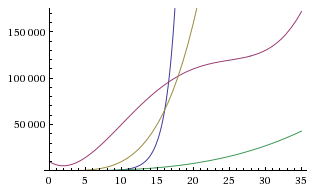
\includegraphics[width=5cm]{images/fourgraphs}
    \begin{flushleft}
    \relscale{0.5}
    \begin{itemize}
      \item $2^x$
      \item $x^4$
      \item $(x-20)^4+10(x-30)^3+120,000$
      \item $x^3$
    \end{itemize}
      
    \end{flushleft}
  \end{column}
\end{columns}



\end{frame}


\section{Времеви ресурс}


\begin{frame}
\centerline{Ресурси, нужни за изпълнението на алгоритъм,}
\centerline{като фунцкия на ``обема'' на входа}
\end{frame}



\begin{frame}[fragile]
\frametitle{Константно време}


\begin{columns}[t]
  \begin{column}{0.6\textwidth}
\begin{remark}[]
\relscale{0.75}
  \begin{lstlisting}[mathescape]
  do something simple;
  do something else simple;
  do something simple;
  \end{lstlisting}
\end{remark}

\begin{flushleft}
\relscale{0.65}
\begin{lstlisting}
//int a[n];
cin >> i;
cout << "a[" << i 
     << "]=" << a[i] <<endl;
\end{lstlisting}
\end{flushleft}


  \end{column}
  \begin{column}{0.4\textwidth}

   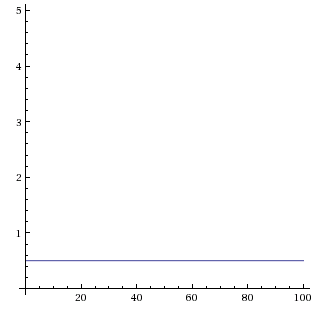
\includegraphics[width=5cm]{images/constantf}
    \begin{flushleft}
    \relscale{0.5}
    \begin{remark}
      Времето за изпълнение не се изменя с увеличаване на $n$.

      $T_P(n) \in \mathcal{O}(1);$
    \end{remark}
      
    \end{flushleft}


  \end{column}
\end{columns}




\end{frame}



\begin{frame}[fragile]
\frametitle{Линейно време}


\begin{columns}[t]
  \begin{column}{0.6\textwidth}
\begin{remark}[]
\relscale{0.75}
  \begin{lstlisting}[mathescape]
  $\forall x \in Input$ do 
      something with 
      constant time complexity;
  \end{lstlisting}
\end{remark}

\begin{flushleft}
\relscale{0.65}
\begin{lstlisting}
int maxi = 0;
for (int i = 1; i < n; i++)
{ 
  if (a[i] > a[maxi]) 
    maxi = i; 
}
\end{lstlisting}
\end{flushleft}

\begin{remark}
\relscale{0.5}
  Време за една итерация, $c$,

  Време за 3 итерации, $3\times c$.
\end{remark}


  \end{column}
  \begin{column}{0.4\textwidth}

   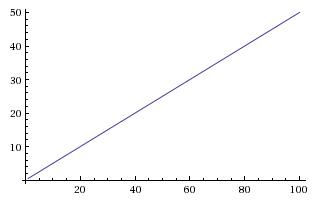
\includegraphics[width=5cm]{images/linearf}
    \begin{flushleft}
    \relscale{0.5}
    \begin{remark}
      Времето за изпълнение нараства линейно с увеличаване на $n$.
 
      $T_P(n) \in \mathcal{O}(n);$
    \end{remark}
      
    \end{flushleft}


  \end{column}
\end{columns}

\end{frame}





\begin{frame}[fragile]
\frametitle{Квадратно време}


\begin{columns}[t]
  \begin{column}{0.6\textwidth}
\begin{remark}[]
\relscale{0.75}
  \begin{lstlisting}[mathescape]
  $\forall x \in Input$ do 
      something with 
      linear time complexity;
  \end{lstlisting}
\end{remark}

\begin{flushleft}
\relscale{0.65}
\begin{lstlisting}
for (int i = 0; i < n; i++)
  for (j = i+1; j < n; j++)
  {
    if (a[i] == a[j]) 
      cout << "Duplicate!";
  }
\end{lstlisting}
\end{flushleft}

\begin{remark}
\relscale{0.5}
  при n=3,

  Време за една итерация, $3 \times c$,

  Време за 3 итерации, $3\times 3 \times c$`'.
\end{remark}


  \end{column}
  \begin{column}{0.4\textwidth}

   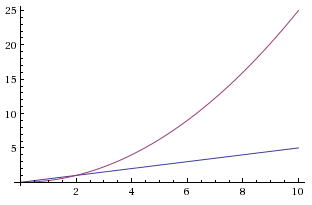
\includegraphics[width=5cm]{images/quadraticf}
    \begin{flushleft}
    \relscale{0.5}
    \begin{remark}
      Времето за изпълнение нараства квадратно с увеличаване на $n$.

      $T_P(n) \in \mathcal{O}(n^2);$
    \end{remark}
      
    \end{flushleft}


  \end{column}
\end{columns}

\end{frame}


\begin{frame}
\centerline{Има ли нещо по-лошо от полиномиалната функция?}

\begin{center}
  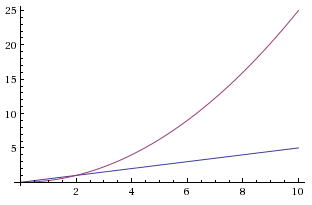
\includegraphics[width=5cm]{images/quadraticf}
\end{center}
\end{frame}


\begin{frame}[fragile]
\frametitle{Екпоненциално време}

\vspace{-30px}

\begin{columns}[t]
  \begin{column}{0.6\textwidth}
\begin{remark}[]
\relscale{0.75}
  \begin{lstlisting}[mathescape]
  k times do 
      something with 
      complexity $\mathcal{O}(k^{n-1})$;
  \end{lstlisting}
\end{remark}

\begin{flushleft}
\relscale{0.65}
\begin{lstlisting}
int fib (int n)
{
  if (n <= 1) return n;
  return fib (n-1) + fib (n-2);
}
\end{lstlisting}
\end{flushleft}




  \end{column}
  \begin{column}{0.4\textwidth}

   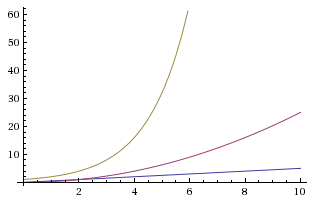
\includegraphics[width=5cm]{images/exponential}
    \begin{flushleft}
    \relscale{0.5}
    \begin{remark}
      Времето за изпълнение нараства експоненциално с увеличаване на $n$.

      $T_P(n) \in \mathcal{O}(a^n);$
    \end{remark}
      
    \end{flushleft}


  \end{column}
\end{columns}

\end{frame}


\begin{frame}[fragile]
\frametitle{n-то число на Фибоначи}

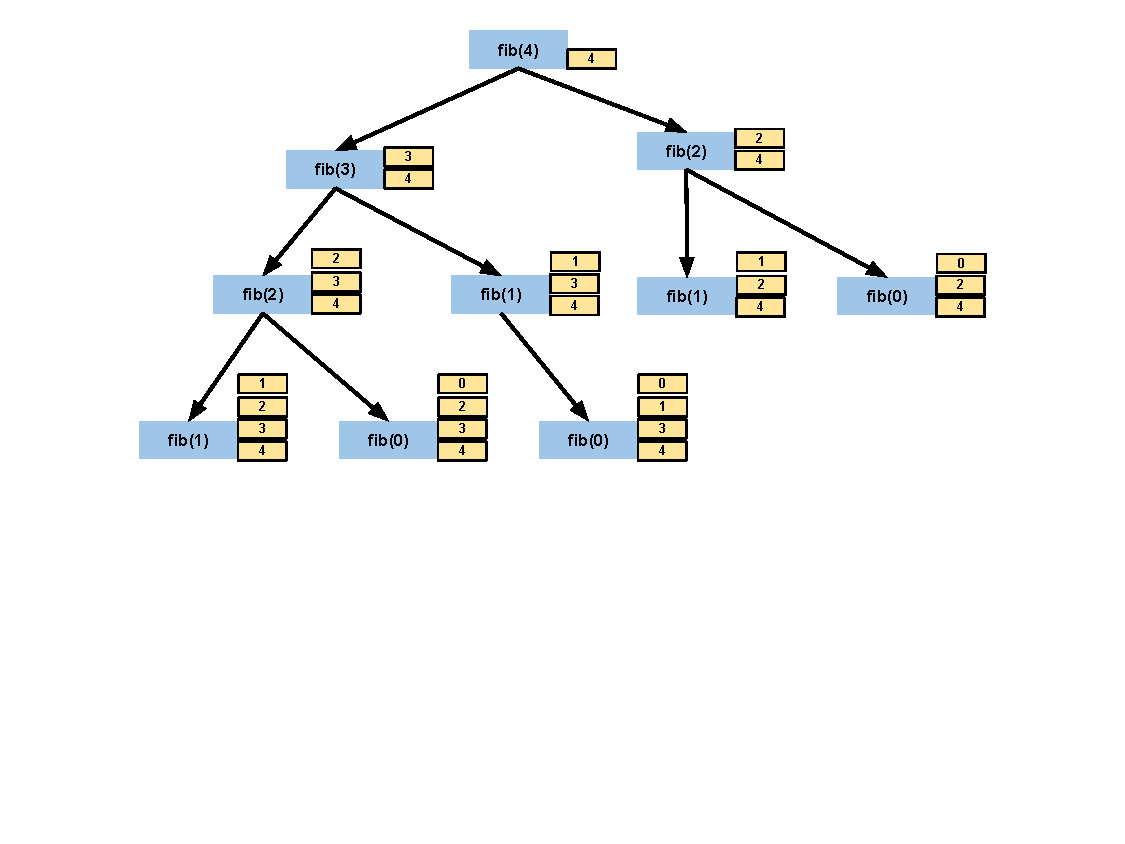
\includegraphics[width=12cm]{images/fib_stack}

\vspace{-100px}

\begin{flushleft}
\relscale{0.55}
\begin{lstlisting}
int fib_n (int n)
{
  if (n <= 1)
    return 1;
  return fib_n(n-2) + fin_n(n-1);
}
\end{lstlisting}  
\end{flushleft}


\end{frame}


\begin{frame}[fragile]
\frametitle{n-то число на Фибоначи за линейно време}


\begin{flushleft}
\relscale{0.85}
\begin{lstlisting}
int fib_n (int n)
{
  int a = 0, b = 1;
  while (n > 0)
  { //(a,b) -> (b,a+b)
    b += a; 
    a = b - a;
    n--;
  }
  return a;
}
\end{lstlisting}  
\end{flushleft}


\end{frame}


\begin{frame}
\centerline{Има ли нещо между линейното и константното?}

\begin{center}
  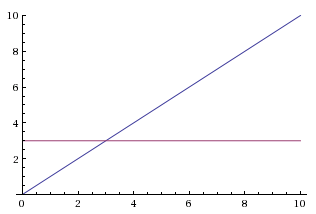
\includegraphics[width=5cm]{images/linearandconst}
\end{center}
\end{frame}

\begin{frame}[fragile]
\frametitle{Логаритмично време}

\vspace{-30px}

\begin{columns}[t]
  \begin{column}{0.6\textwidth}
\begin{remark}[]
\relscale{0.75}
  \begin{lstlisting}[mathescape]
  
    do something simple;
    solve a 
      two times simpler sub-problem;

  \end{lstlisting}
\end{remark}

\begin{flushleft}
\relscale{0.65}
\begin{lstlisting}
bool find (int x, int arr[], int n)
//arr is ordered
{
  if (n == 0)
    return false;

  if (x >= arr[n/2])
    return x==arr[n/2] || 
           find (x,arr+ceil(n/2.0),n/2);

  return find (x,arr,n/2);


}
\end{lstlisting}
\end{flushleft}




  \end{column}
  \begin{column}{0.4\textwidth}

   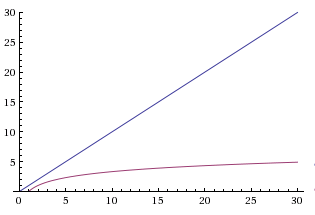
\includegraphics[width=5cm]{images/logf}
    \begin{flushleft}
    \relscale{0.5}
    \begin{remark}
      Сложността на проблема намалява двойно на всяка стъпка.
      Времето за изпълнение нараства логаритмично с увеличаване на $n$.

      $T_P(n) \in \mathcal{O}(log_2(n));$
    \end{remark}
      
    \end{flushleft}


  \end{column}
\end{columns}

\end{frame}

\begin{frame}
\centerline{Благодаря за вниманието!}
\end{frame}


\end{document}


\begin{columns}[t]
  \begin{column}{0.2\textwidth}

  \end{column}
  \begin{column}{0.8\textwidth}

  \end{column}
\end{columns}
